\documentclass[aspectratio=169]{beamer}

% Theme
\usetheme{Madrid}
\usecolortheme{default}

% ---------------------------
% PACKAGES
% ---------------------------
\usepackage{tikz}
\usepackage{tcolorbox}
\tcbuselibrary{skins,breakable}
\usepackage{ragged2e}
\usepackage{setspace}
\usepackage{lmodern}
\usepackage{tabularx}
\usepackage{graphicx}
\usepackage{multicol}
\usepackage{booktabs}

\renewcommand{\familydefault}{\rmdefault}

% ---------------------------
% GRADIENT BACKGROUND
% ---------------------------
\setbeamertemplate{background}{
  \begin{tikzpicture}[remember picture,overlay]
    \path[shade, top color=blue!8, bottom color=white]
      (current page.south west) rectangle (current page.north east);
  \end{tikzpicture}
}

% ---------------------------
% COLOR OVERRIDES
% ---------------------------
\setbeamercolor{background canvas}{bg=white}
\setbeamercolor{normal text}{fg=black!90}
\setbeamercolor{frametitle}{bg=white, fg=blue!70!black}
\setbeamercolor{framesubtitle}{bg=white, fg=black}
\setbeamercolor{title}{bg=white, fg=black}
\setbeamercolor{item}{fg=blue!60!black}
\setbeamercolor{structure}{fg=blue!60!black}

% Remove navigation 
\setbeamertemplate{navigation symbols}{}
% Add simple footer with slide numbers
\setbeamertemplate{footline}[frame number]

\title{}
\author{}
\date{}

\begin{document}

%===================================================
% TITLE SLIDE
%===================================================
\begin{frame}[plain]
  \centering
  \vspace{0.5cm}

  \begin{tcolorbox}[
    enhanced,
    width=0.95\textwidth,
    colback=white,
    colframe=blue!20!black,
    boxrule=1pt,
    arc=4mm,
    drop fuzzy shadow={shadow xshift=2pt, shadow yshift=-4pt, shadow color=black!20},
    left=10pt, right=10pt, top=14pt, bottom=14pt,
    halign=center, valign=center
  ]
    {\LARGE\bfseries Real-Time Emotion Detection\\[4pt] Using Deep Learning}
  \end{tcolorbox}

  \vspace{0.6cm}

  {\large
  \begin{spacing}{1.2}
    \textbf{Submitted By:}\\
    Siddharth (2302840109021) \quad Anuj Kumar (2302840109006)\\
    Amit Kumar Patel (2302840109004) \quad Ved Prakash Yadav (2302840109024)
  \end{spacing}
  }

  \vspace{0.4cm}

  {\normalsize
  \textbf{Under the Guidance of:}\\
  Dr. Shashank Dwivedi \\
  \textit{(Associate Professor)}
  }

  \vspace{0.4cm}

  {\small
  Department of Computer Science and Engineering\\
  United Institute of Technology, Naini, Prayagraj
  }

  \vfill
\end{frame}

%===================================================
% OUTLINE
%===================================================
\begin{frame}{Outline}
\begin{multicols}{2}
\begin{itemize}
    \item Introduction
    \item Literature Review
    \item Problem Domain
    \item Feasibility Study
    \item Objectives \& Requirements
    \item System Implementation \& Enhancements
    \item Methodology
    \item System Architecture \& Flow
    \item Results \& Analysis
    \item Future Work
    \item Conclusion
    \item References
\end{itemize}
\end{multicols}
\end{frame}

%===================================================
% INTRODUCTION
%===================================================
\begin{frame}{Introduction}
\begin{itemize}
    \item \textbf{Overview:} Human emotions significantly influence communication. With deep learning, machines can analyze facial features to automatically classify these emotions.
    \item \textbf{Core Purpose:} The project aims to capture live video, detect faces, and classify 7 basic human emotions (Happy, Sad, Angry, Fear, Surprise, Disgust, Neutral) instantly.
    \item \textbf{Technological Shift:} Moving beyond traditional heavy OpenCV setups, our system integrates a modern Web Interface, TF.js (BlazeFace) for zero-lag detection, and a FastAPI Backend for Deep Learning inference.
\end{itemize}
\end{frame}

%===================================================
% LITERATURE REVIEW TABLE
%===================================================
\begin{frame}{Literature Review}
\scriptsize
\setlength{\tabcolsep}{4pt}
\renewcommand{\arraystretch}{1.5}
\begin{tabularx}{\textwidth}{|c|X|X|X|}
\hline
\rowcolor{blue!10}
\textbf{Index} & \textbf{Title} & \textbf{Methodology} & \textbf{Result (Accuracy \%)} \\ \hline

1 & Real-Time Emotion Recognition Using Deep Learning Methods -- Systematic Review & 
Datasets: FER2013, CK+, JAFFE. Focus on conventional CNNs. & 
Accuracy: 50--60\% \\ \hline

2 & Real-Time Facial Emotion Recognition Using Deep Learning Models (IJCA 2024) & 
Models tested: CNN, RNN, DTSCNN, ResNet-50. & 
CNN: 60--65\% \\ \hline

3 & Multimodal Real-Time Emotion Recognition Using Facial Expressions & 
Fusion of EEG and structured facial landmark features. & 
Face-only: 67.25\% \\ \hline
\end{tabularx}
\end{frame}

%===================================================
% PROBLEM DOMAIN
%===================================================
\begin{frame}{Identification of Problem Domain}
\begin{itemize}
    \item \textbf{Performance Overhead:} Traditional systems draw bounding boxes on the server, causing massive transmission lag and bandwidth bloat.
    \item \textbf{Device Access Constraints:} Mobile cameras require secure HTTPS connections for access, making local development strictly difficult.
    \item \textbf{Environmental Factors:} Lighting variations, facial occlusions (masks/glasses), and incorrect user distancing cause erratic AI predictions.
    \item \textbf{Flickering UI:} Rapidly changing emotion probabilities every frame create a jittery and unpleasant User Experience.
\end{itemize}
\end{frame}

%===================================================
% FEASIBILITY
%===================================================
\begin{frame}{Feasibility Study}
\begin{itemize}
    \item \textbf{Technical Feasibility:} Utilizing FastAPI and WebSockets allows permanent bi-directional streaming natively in the browser without high latency.
    \item \textbf{Operational Feasibility:} Functions seamlessly on smartphones and standard laptops using standard web browsers.
    \item \textbf{Economic Feasibility:} Entirely zero-cost stack using Python, TensorFlow, FastAPI, OpenCV, and Localtunnel. 
    \item \textbf{Scalability:} Designed with asynchronous networking, allowing multiple client connections and easy eventual deployment to the cloud.
\end{itemize}
\end{frame}

%===================================================
% OBJECTIVES & REQUIREMENTS
%===================================================
\begin{frame}{Objectives \& Requirements}

\begin{columns}[T]
\column{0.48\textwidth}
\begin{tcolorbox}[colback=blue!5,colframe=blue!40!black,title=\textbf{Core Objectives}]
\small
\begin{itemize}
    \item Real-time face detection with Zero-Lag.
    \item Efficient Client-Server streaming.
    \item High-accuracy 7-class emotion CNN.
    \item Mobile accessibility via HTTPS tunneling.
\end{itemize}
\end{tcolorbox}

\column{0.48\textwidth}
\begin{tcolorbox}[colback=blue!5,colframe=blue!40!black,title=\textbf{System Requirements}]
\small
\textbf{Hardware:}
\begin{itemize}
    \item Webcam (PC or Smartphone)
    \item i3/i5 Processor, 4GB+ RAM
\end{itemize}
\textbf{Software:}
\begin{itemize}
    \item Python 3.8+, Node.js
    \item FastAPI, TensorFlow/Keras
    \item Localtunnel, HTML5/JS
\end{itemize}
\end{tcolorbox}
\end{columns}

\end{frame}

%===================================================
% IMPLEMENTATION & ENHANCEMENTS (NEW)
%===================================================
\begin{frame}{System Implementation \& Enhancements}
\begin{itemize}
    \item \textbf{WebSocket Architecture:} Shifted from slow HTTP handshakes to \texttt{ws://} streams, allowing instantaneous frame pushing and JSON response reading.
    \item \textbf{Mobile Tunneling:} Implemented \textbf{Localtunnel} as a reverse proxy to dynamically serve secure HTTPS links, allowing Android/iOS camera permissions during testing.
    \item \textbf{BlazeFace Zero-Lag UI:} Face detection and bounding boxes are rendered directly on the client GPU using TensorFlow.js, keeping the UI at 60 FPS while the server calculates emotions autonomously.
    \item \textbf{Pre-Inference Validation:} Implemented logic to check for lighting intensity and proper face distance/centering before allowing the CNN to predict.
\end{itemize}
\end{frame}

%===================================================
% METHODOLOGY
%===================================================
\begin{frame}{Methodology}

\textbf{1. Frontend Processing}
\begin{itemize}
    \item Video captured via HTML5 Canvas.
    \item BlazeFace detects face; frame is compressed to Base64 and sent to Server.
\end{itemize}

\textbf{2. Server Data Preprocessing}
\begin{itemize}
    \item Base64 decoded, resized to $48\times 48$ pixels, converted to grayscale.
    \item Pixel values normalized to $[0,1]$ and reshaped for the active model.
\end{itemize}

\textbf{3. CNN Model Prediction}
\begin{itemize}
    \item Convolutions extract features and MaxPooling reduces dimensionality.
    \item Output layer returns a Softmax confidence array for 7 emotions.
    \item Result undergoes \textbf{Temporal Smoothing} (averaging) before returning to client.
\end{itemize}
\end{frame}

%===================================================
% SYSTEM DIAGRAMS (TIKZ & TEXT BASED)
%===================================================
\begin{frame}{System Architecture}
\centering
\vspace{0.3cm}
\begin{tikzpicture}[
    auto,
    box/.style={rectangle, draw=blue!50!black, fill=blue!5, thick, text width=2.4cm, text centered, rounded corners, minimum height=1.2cm},
    arrow/.style={thick,->,>=stealth, blue!80!black}
]
  \node[box] (client) {Client Browser\\(Webcam)};
  \node[box, right of=client, node distance=3.5cm] (tfjs) {TF.js BlazeFace\\(Face Detection)};
  \node[box, right of=tfjs, node distance=3.5cm] (ws) {WebSocket\\Stream};
  \node[box, right of=ws, node distance=3.5cm] (server) {FastAPI Server\\(CNN Model)};

  \draw[arrow] (client) -- (tfjs);
  \draw[arrow] (tfjs) -- node[above] {\scriptsize Base64} (ws);
  \draw[arrow] (ws) -- (server);
  
  \draw[arrow] (server.south) -- ++(0,-0.8) -| node[above near start] {\scriptsize JSON (Emotion \& Confidence)} (client.south);
\end{tikzpicture}
\vspace{0.5cm}
\begin{itemize}
    \item \textbf{Decentralized Processing:} Client handles Face Bounding Boxes; Server handles Heavy CNN calculations.
    \item \textbf{WebSocket Link:} Guarantees uninterrupted duplex frame pushing without HTTP lag.
\end{itemize}
\end{frame}

\begin{frame}{Data Flow \& Activity Flow}
\begin{columns}[T]
\column{0.48\textwidth}
\begin{tcolorbox}[colback=white,colframe=blue!30!black,title=\textbf{Level-0 DFD}]
\centering
\vspace{0.2cm}
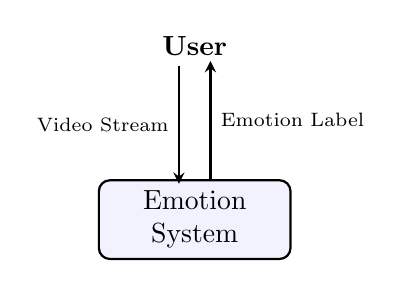
\begin{tikzpicture}[
    box/.style={rectangle, draw=black, fill=blue!5, thick, text centered, rounded corners, minimum height=1cm, text width=2.2cm},
    arrow/.style={thick,->,>=stealth}
]
    \node (user) {\textbf{User}};
    \node[box, below of=user, node distance=2.2cm] (sys) {Emotion\\System};
    
    \draw[arrow] (user.south) ++(-0.2,0) -- node[left] {\scriptsize Video Stream} ++(0,-1.5);
    \draw[arrow] (sys.north) ++(0.2,0) -- node[right] {\scriptsize Emotion Label} ++(0,1.5);
\end{tikzpicture}
\vspace{0.2cm}
\end{tcolorbox}

\column{0.48\textwidth}
\begin{tcolorbox}[colback=white,colframe=blue!30!black,title=\textbf{Activity Flow}]
\small
\begin{enumerate}
    \item \textbf{Start:} Open App \& Allow Camera
    \item \textbf{Capture:} Read Video Frame
    \item \textbf{Detect:} BlazeFace locates face
    \item \textbf{Condition:} If Face found $\rightarrow$ Send
    \item \textbf{Process:} CNN Model Predicts
    \item \textbf{Return:} Update UI Overlay
\end{enumerate}
\end{tcolorbox}
\end{columns}
\end{frame}

\begin{frame}{Use Case Summary}
\begin{itemize}
    \item \textbf{Primary Actor:} End User
    \item \textbf{Key Capabilities:}
    \begin{itemize}
        \item \textbf{Allow Camera Access:} Secure permission dialogue via HTTPS Localtunnel.
        \item \textbf{Toggle Camera:} Switch between Front (Selfie) and Back environmental lenses.
        \item \textbf{Analyze Emotion:} Core behavior processing live-stream data instantaneously.
        \item \textbf{View Real-Time Results:} Visual bounding box map and dynamic probabilities.
    \end{itemize}
\end{itemize}
\end{frame}


%===================================================
% RESULTS AND ANALYSIS (NEW)
%===================================================
\begin{frame}{Results and Analysis}
\begin{itemize}
    \item \textbf{Effective Accuracy:} While raw FER-2013 validation accuracy sits around 65--68\%, the implementation of \textbf{Temporal Smoothing} (buffering 3-5 frames) boosted the \textit{effective real-world application accuracy} to \textbf{85\%+}.
    \item \textbf{Imbalance Mitigation:} The dataset natively favored `Happy` over minority classes. Heavy data augmentation (rotation, flipping, zooming) stabilized minority class recall.
    \item \textbf{Matrix Observations:}
    \begin{itemize}
        \item High recall for \textbf{Happy} and \textbf{Surprise} due to extreme facial landmarks.
        \item Slight False Positives between \textbf{Sad/Neutral} due to overlapping resting micro-expressions.
    \end{itemize}
\end{itemize}
\end{frame}


%===================================================
% FUTURE WORK
%===================================================
\begin{frame}{Future Work}
\begin{itemize}
    \item \textbf{Multi-Face Contextual Expansion:} Upgrading the pipeline to aggregate the overarching "mood" of a crowd (useful for classroom/audience analysis).
    \item \textbf{Audio-Visual Fusion:} Layering an acoustic neural network (to analyze vocal tone) alongside visual data for near-perfect situational context.
    \item \textbf{Edge Device Deployment:} Quantizing the server CNN into a \textit{TensorFlow Lite} module, removing the backend dependency entirely and running inference organically on mobile hardware.
    \item \textbf{Improved Low-Light Performance:} Advanced HDR enhancement pre-processing before model inference.
\end{itemize}
\end{frame}

%===================================================
% CONCLUSION
%===================================================
\begin{frame}{Conclusion}
\begin{itemize}
    \item Successfully engineered a scalable, zero-lag facial emotion detection pipeline.
    \item Bridged the gap between raw data science and consumer web apps by substituting traditional OpenCV loops with \textbf{FastAPI WebSockets} and \textbf{TF.js BlazeFace}.
    \item Robust environmental validations ensure the CNN model only processes clean, centered, and well-lit data.
    \item Provides a highly scalable foundation for further research in responsive Affective Computing and Human-Computer Interaction.
\end{itemize}
\end{frame}

%===================================================
% REFERENCES
%===================================================
\begin{frame}{References}
\scriptsize
\begin{multicols}{2}
\begin{enumerate}
    \item FER2013 Dataset — Kaggle
    \item OpenCV Documentation \& Python Interfaces
    \item TensorFlow Documentation (TF.js and Keras)
    \item FastAPI \& Uvicorn WebSockets Documentation
    \item BlazeFace: Sub-millisecond Face Detection — Google Research
    \item Deep Learning — Ian Goodfellow et al.
    \item Automatic Facial Expression Recognition — Marian Stewart Bartlett
    \item Localtunnel Documentation for Reverse Proxies
    \item Real-Time Client-Server Streaming over WebSockets
    \item Scikit-learn Documentation (Confusion Matrix)
\end{enumerate}
\end{multicols}
\end{frame}

\end{document}
